\subsection*{Fibers}{}

\begin{frame}{Methods Overview}{Methods and algorithms}
     \begin{description}
        \item $\square$ \alert{Fiber cycle breaking}
        \item $\square$  Visit sequences
        \item $\square$  SCC chunk scheduling
    \end{description}
\end{frame}

\note[itemize]{
\item Next, we are going to talk about fiber cycles 
}

\begin{frame}{Fiber Construction}{Informal Definition: Beyond the scope of this presentation}

\small
\begin{itemize}
    \item A construction that expresses the semantics of \emph{remote attribute grammars} in \emph{classical terms}
    \item Objects \alert{implicitly} carry separate values for the fields is like a \alert{rope} which can be separated into the individual fibers
    \item This yields an improper attribute grammar with an infinite number of attributes
    \item \emph{fiber approximation} fixes that (which then may include \alert{fiber cycles})
\end{itemize}

\begin{center}
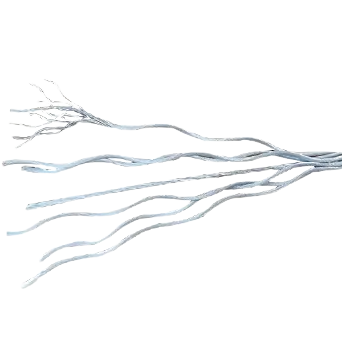
\includegraphics[scale=0.2]{rope-fiber.png}
\end{center}
    
\end{frame}

\note[itemize]{
    \item I am intentionally not going into details of fiber-construction because it would be a disservice to remote attribute grammar paper
    \item Basically, it expresses the semantics of remote attribute grammars in classical terms
    \item It is called \enquote{fibers} because objects implicitly carry separate values for the fields and it is like a rope that can be separated into individual fibers
    \item But fiber-construction yields an improper attribute grammar with an infinite number of attributes
    \item Then fiber-approximation fixes that but it then may include \alert{fiber-cycles}
}


% 

\begin{frame}{Fiber Cycle Breaking}{Benign fiber cycles are okay for scheduling}

\alert{Fiber attributes} guide the scheduler and have no run-time significance

\newlinevspace

\begin{itemize}
    \item % some cycles are benine because they only consist of fiber attruibyres
In RAG, some cycles can be ignored because they entirely involve so-called fiber attributes

\newlinevspace

%  in existing APS systsme, they can be scheduled using a hack that added new attributes UP and DOWN to break cycles
%  in this work we found we didn't need this hack, we found that we can handle them generalkly because they are monotone
% fiber attributes
    \item In CAG (or CRAG), some cycles may \alert{carry value} and this will have run-time significance
\end{itemize}
\end{frame}

\note[itemize]{
\item Even in a remote attribute grammar that is non-circular we may have pure fiber cycles and it's okay.
\item Fiber cycles are different between remote attribute grammar and circular remote attribute grammar because in the latter case, they may carry value
}



\begin{frame}{Fiber Cycle Breaking}{Issue with existing static scheduler}

Previously in RAG:
\begin{itemize}
    \item For every non-terminal whose fibered attributes take part in the cycle, created two \alert{AST nodes} called up and down and connected all nodes to these to break cycles and \alert{preserve only UP followed by DOWN}.
\end{itemize}


\end{frame}

\note[itemize]{
\item Previously for remote attribute grammars, fiber cycles were broken and to do that two artificial attributes called UP and DOWN would be created. This introduced a lot of implementation complexity
\item To fix that we wrote a new algorithm that treats all attributes as either UP or DOWN and it simplifies fiber cycle breaking
}



% kill this
% \begin{frame}{Fiber Cycle Breaking}{Validated with RAG!}

% \alert{Drop-in replacement} algorithm was successful in APS.

% \begin{itemize}
%     \item Validated the algorithm against \alert{previous APS codes} that contained only fiber cycles
% \end{itemize}

% \end{frame}

% \note[itemize]{
% \item We tested the fiber cycle breaking algorithm against APS examples that contained only fiber cycles
% \item And it was successful 
% }



\begin{frame}{Fiber Cycles Are Monotone}{CRAG static scheduler can handle fiber cycles}
    \textbf{But} this turned out to be \alert{unnecessary} because fiber dependencies are \alert{monotone} and can be handled by the new CRAG scheduler, so this change was not necessary. 

\newlinevspace
Welcome outcome.
    
\end{frame}

\note[itemize]{
\item But the whole fiber cycle breaking change turned out to be unnecessary and not needed because fiber cycles are monotone and can be handled by the CRAG static scheduler
\item This is welcome news because the simpler the implementation, the better
}